\documentclass[10pt]{beamer}

\usetheme{sthlm}

%%%% STHLM
\usepackage{metalogo}
%\usepackage[utf8]{inputenc}
\usepackage{%
	booktabs,
	datetime,
	dtklogos,
	pgfplots,
	ragged2e,
	tabularx,
	wasysym
}
\usepackage[scale=2]{ccicons}
%%%% /STHLM


\usepackage{nameref}
\makeatletter
\newcommand*{\currentname}{\@currentlabelname}
\makeatother

\newcommand*{\footnotedef}[2]{#1\footnote{\textbf{#1}: #2}}
\newcommand*{\red}[1]{{\color{red}#1}}
\newcommand*{\TODO}{\red{TODO}}
\usepackage{xcolor}

\hypersetup{%
	colorlinks,
	linkcolor=sthlmBlue,
	urlcolor=sthlmBlue,
	linkbordercolor=sthlmBlue,
	pdfborderstyle={/S/U/W 1}
%	linkcolor={red!50!black}
	%linkcolor={196!0!100},
}

% so we don't have 'Figure x.x' on captions
\setbeamertemplate{caption}{\raggedright\insertcaption\par}

\title{Docker-IA}
\subtitle{\large A Docker-based container infrastructure to build the Android Source Code for different Intel Architecture platforms.}
\date{\today}
\author{Jamie Tanna}
% \institute{\href{http://hacksocnotts.co.uk}{Hacksoc Nottingham}
%}

\usepackage{listings}
\lstset{%
	language=bash,
	keepspaces=true,
	basicstyle=\ttfamily
}

\begin{document}

\maketitle

\begin{frame}
	\frametitle{Overview}
	\setbeamertemplate{section in toc}[sections numbered]
	\tableofcontents
	% \tableofcontents[hideallsubsections]
\end{frame}

\section{Docker-IA}
\subsection{What is Docker-IA?}

\begin{frame}
	\frametitle{\currentname}

	\begin{figure}[c]
		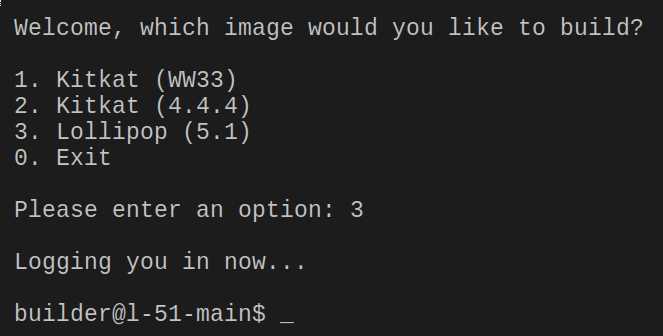
\includegraphics[width=0.6\textwidth]{./images/projects-docker_android_ia.png}
		\\
	\end{figure}

	\begin{itemize}
		\item An system for easily building the Android sources
		\item Contain dependencies
			\begin{itemize}
				\item Different devices
				\item Different Android versions
			\end{itemize}

		\item Easily accessible
			\begin{itemize}
				\item Samba, nginx
			\end{itemize}

		\item Get notified when builds are complete - along with link to the image
		\item Only one copy of all the source code
			\begin{itemize}
				\item \texttt{repo init --reference /path/to/sources}
				\item Regularly sync'd
			\end{itemize}
	\end{itemize}
\end{frame}

\subsection{Rationale for the project}
\begin{frame}
	\frametitle{\currentname}

	\begin{itemize}
		\item Working on a large-scale tablet project for a retailer
		\item Dependencies for KK vs L

		\item Replace \href{http://buildbot.net}{BuildBot}
			\begin{itemize}
				\item 40 minute \textbf{clean} builds
				\item Network transfer times
			\end{itemize}
		\item Reuse previous builds
			\begin{itemize}
				\item Quick iterations
				\item Play around with the code ourselves
			\end{itemize}
		\item Why Docker vs LXC vs VMs?
	\end{itemize}
\end{frame}

\subsection{Wrapping Docker}
\begin{frame}
	\frametitle{\currentname}

	\begin{figure}[c]
		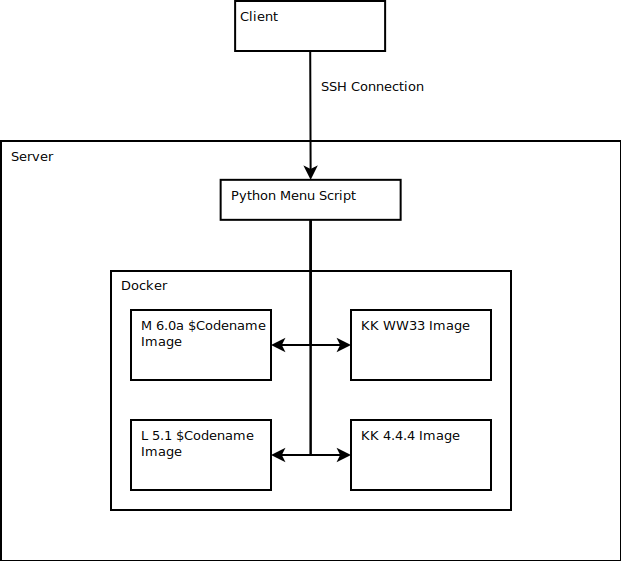
\includegraphics[width=0.6\textwidth]{./images/docker-architecture.png}
		\\Architecture Overview of Docker-IA
	\end{figure}
\end{frame}

\begin{frame}
	\frametitle{\currentname}

	\begin{figure}[c]
		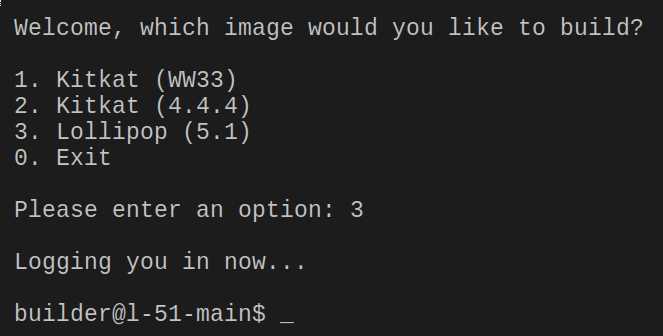
\includegraphics[width=0.6\textwidth]{./images/projects-docker_android_ia.png}
		\\
	\end{figure}

	\begin{itemize}
		\item Friendly menu to log into images
			\begin{itemize}
				\item Compared to \texttt{docker run -v /path/to/volume:/android -v /path/to/fifo:/run/email-fifo -ti kk-intel-444 /bin/bash}
				\item Team-wide usage
			\end{itemize}

		\item Prevent multiple users from modifying the same sources
		\begin{itemize}
			\item \href{http://tmux.github.io/}{tmux}
			\item \href{https://pypi.python.org/pypi/tmuxp}{\texttt{tmuxp}}
		\end{itemize}
	\end{itemize}
\end{frame}

\subsection{Potential Extensions}
\begin{frame}
	\frametitle{\currentname}

	\begin{itemize}
		\item Inform users when:
			\begin{itemize}
				\item Users are logged in
				\item Builds are in progress
			\end{itemize}

		\item Add more automation:
			\begin{itemize}
				\item Create new environments
				\item Save built images  
			\end{itemize}

		\item Scale resource usage better
	\end{itemize}
\end{frame}

\subsection{Project Outcomes}

\begin{frame}
	\frametitle{\currentname}

	\begin{itemize}
		\item Learning:
			\begin{itemize}
				\item \href{https://pypi.python.org/pypi/tmuxp}{\texttt{tmuxp}}
				\item Docker
				\item The Android Sources build process
			\end{itemize}

		\item Enhanced understanding of Bash, the Linux filesystem and Python
		\item Adopted in said retailer's infrastructure
	\end{itemize}
\end{frame}

\end{document}
